\newpage
\section{Общие сведения о системе}
\subsection{Запуск приложения}

\tmis~работает через Web-интерфейс и не требует установки на клиентской рабочей станции никакого дополнительного программного обеспечения. Единственным обязательным условием является наличие установленного Web-браузера, который, как правило, включен по умолчанию в состав любой операционной системы.

Для запуска приложения следует использовать соответствующий ярлык на рабочем столе. При его отсутствии можно запустить Web-браузер и в адресной строке ввести адрес сервера, через который осуществляется доступ к системе. Адрес сервера можно уточнить у администратора системы. 

\subsection{Вход в систему}

После запуска \tmis , необходимо выполнить вход в систему, используя персональный идентификатор пользователя и пароль. Процедура входа в систему называется \dm{авторизацией}. \label{auth}

Перед первым входом в систему необходимо получить персональный идентификатор пользователя (логин) и пароль у администратора системы.

\begin{vnim}
 Персональный идентификатор и пароль предназначены для индивидуального доступа в систему. Никогда не сообщайте их третьим лицам!
\end{vnim}
 
Следует ввести идентификатор пользователя и пароль в соответствующие поля на странице входа в систему (Рисунок \ref{img_gen_login}) и нажать кнопку \btn{Войти}. 

\begin{figure}[!ht]\centering
 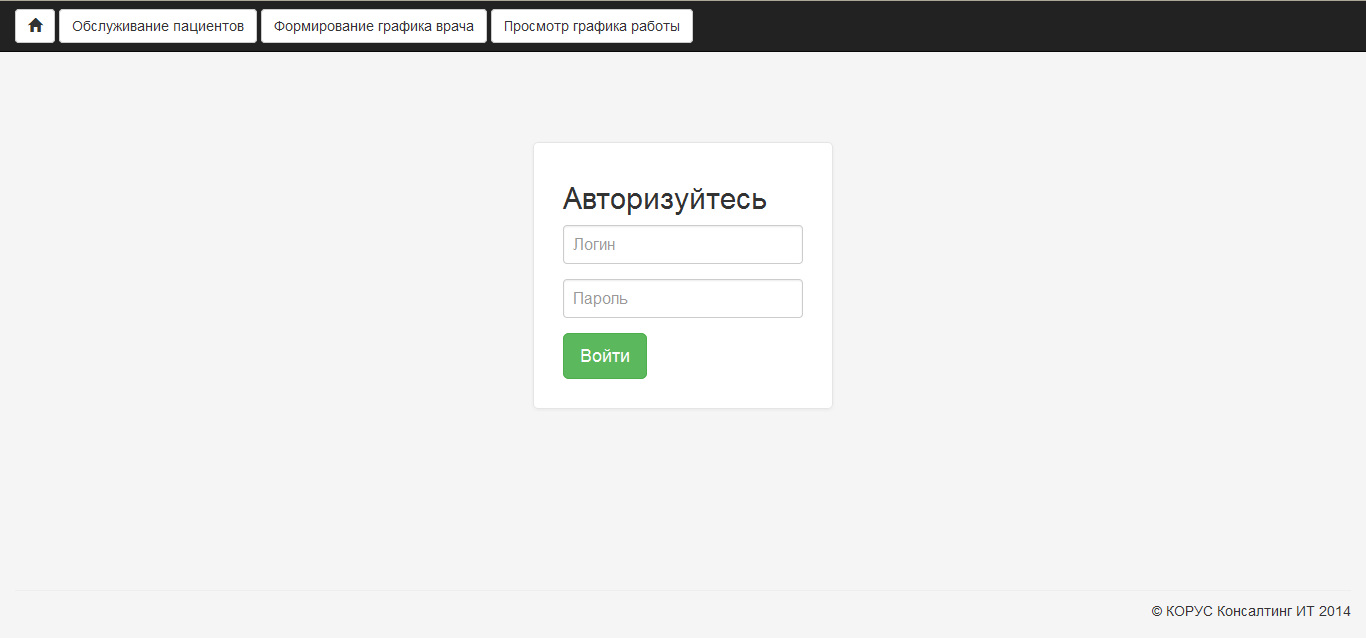
\includegraphics[width = 1\textwidth ,keepaspectratio]{gen_login}
 \caption{Страница авторизации}
 \label{img_gen_login}
\end{figure} 

В случае, если у пользователя имеется несколько ролей, откроется страница выбора роли (Рисунок \ref{img_gen_role}), где  нужно выбрать роль, под которой будет осуществляться работа в текущий момент, из раскрывающегося списка  и нажать кнопку \btn{Выбрать}. В случае, если у пользователя имеется только одна роль, она будет выбрана автоматически. Откроется главная страница системы (Рисунок \ref{img_gen_main}). В зависимости от выбранной роли пользователя и доступных ему функций, внешний вид страницы может отличаться.  

\begin{figure}[!ht]\centering
 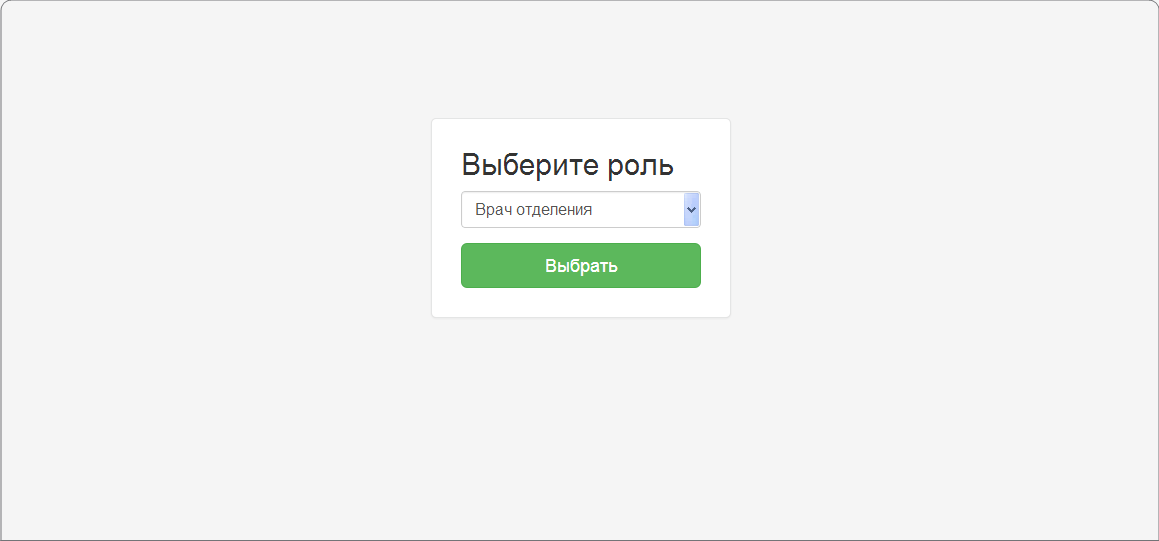
\includegraphics[width = 1\textwidth ,keepaspectratio]{gen_role}
 \caption{Страница выбора роли пользователя}
 \label{img_gen_role}
\end{figure} 

\begin{figure}[!ht]\centering
 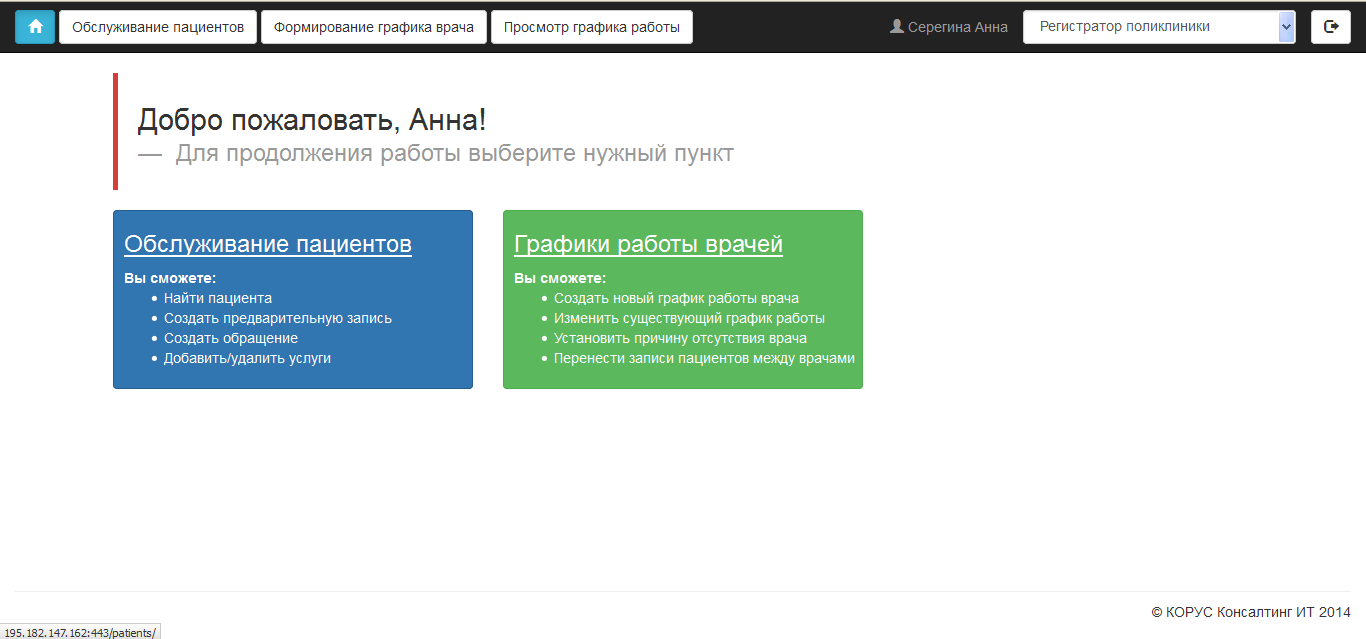
\includegraphics[width = 1\textwidth ,keepaspectratio]{gen_main}
 \caption{Главная страница системы}
 \label{img_gen_main}
\end{figure} 

Если идентификатор пользователя или пароль были введены неверно, то вход в систему не будет осуществлен, а над полем для ввода имени пользователя появится сообщение об ошибке <<Неверное имя пользователя или пароль>> (Рисунок \ref{img_gen_lfail}).

\begin{figure}[!ht]\centering
 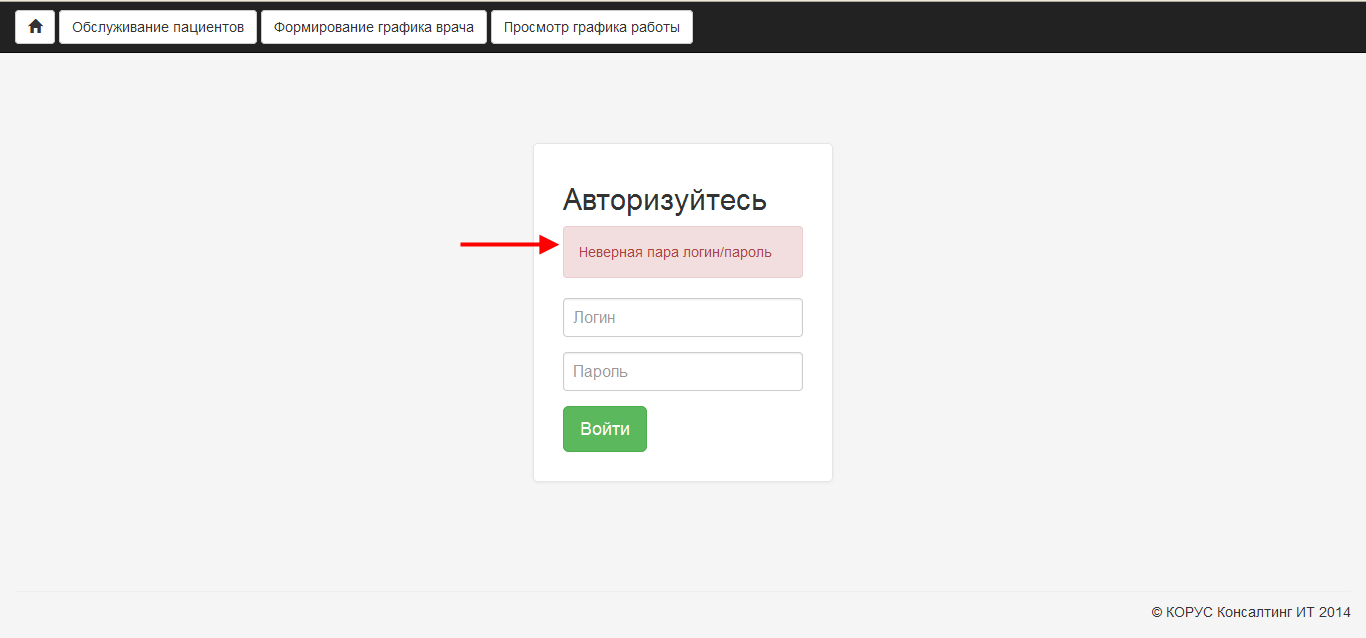
\includegraphics[width = 0.4\textwidth ,keepaspectratio]{gen_lfail}
 \caption{Ошибка авторизации}
 \label{img_gen_lfail}
\end{figure} 

В случае возникновения ошибки необходимо:
\begin{enumerate}
 \item Проверить правильность введенного идентификатора пользователя;
 \item Проверить правильность введенного адреса для подключения (если вводился вручную);
 \item Проверить язык ввода;
 \item Проверить состояние клавиши \keys{CapsLock} на клавиатуре и выключить ее при необходимости;
 \item Если в пароле присутствуют цифры, проверить состояние клавиши \keys{NumLock}, включить ее при необходимости;
 \item Повторить попытку авторизации.
\end{enumerate}
 
Если проблема не была решена, нужно обратиться к администратору системы для проверки идентификационных данных.

\ifthenelse{\isnamedefined{assistversion} \OR \isnamedefined{fullversion}}
{
\subsection{Выбор врача для ассистирования}

В случае входа в систему в качестве медсестры-ассистента врача, перед началом работы следует выбрать врача, которому будет осуществляться ассистирование. Страничка выбора врача открывается автоматически сразу после входа в систему (Рисунок \ref{img_gen_assist_log}). 

 \begin{figure}[!ht]\centering
 	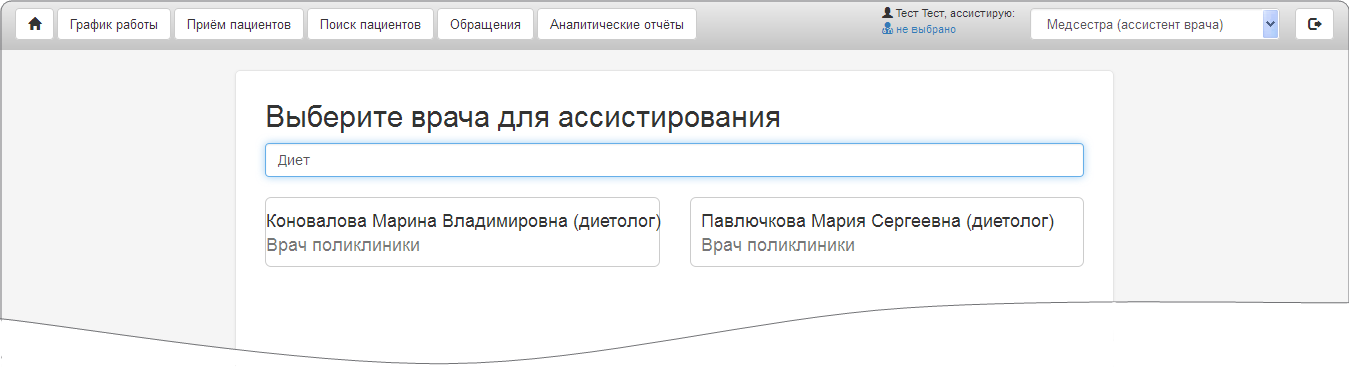
\includegraphics[width = 1\textwidth ,keepaspectratio]{gen_assist_log}
 	\caption{Страница выбора врача для ассистирования}
 	\label{img_gen_assist_log}
 \end{figure} 

В верхней части страницы находится поле поиска \slash фильтрации списка врачей. В данное поле можно ввести часть фамилии или специальность врача. По мере ввода текста в поле, список врачей будет фильтроваться в соответствии с условиями поиска -- в списке останутся только врачи, чья специальность или фамилия содержат введенное буквосочетание. Для возврата к полному списку врачей следует очистить поле поиска. Для перемещения по списку можно использовать полосу прокрутки в правой части списка или колесо мыши.

Когда нужный врач найден в списке, следует щелкнуть по кнопке с его фамилией. Указанный врач будет выбран, и его фамилия появится на панели управления в верхней части страницы, рядом с именем пользователя (Рисунок \ref{img_gen_assist_name}). При этом медсестре становятся доступны те же функции, что и выбранному врачу.

 \begin{figure}[!ht]\centering
 	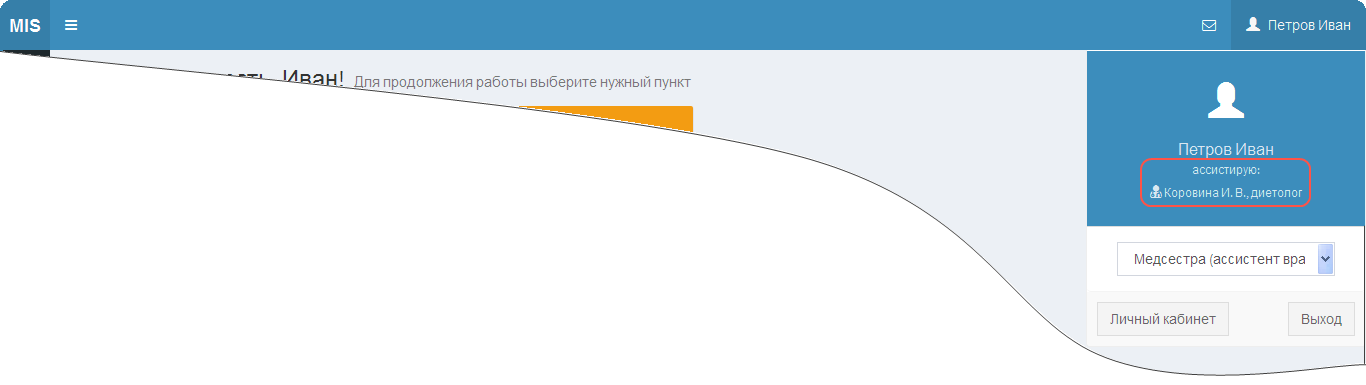
\includegraphics[width = 0.5\textwidth ,keepaspectratio]{gen_assist_name}
 	\caption{Указание фамилии врача для ассистирования}
 	\label{img_gen_assist_name}
 \end{figure}
}{} 
 
\subsection{Завершение работы}

После окончания работы, необходимо выйти из системы. Для этого нужно нажать кнопку 
\includegraphics[scale=0.6]{exit} в правом верхнем углу страницы. Будет осуществлен выход из системы и возврат на страницу авторизации. Если требуется войти в систему под другим именем пользователя, следует пройти процедуру авторизации с новыми идентификационными данными. Если работа с системой завершена, можно закрыть Web-браузер, нажав на кнопку \btn{x} в правом верхнем углу окна или выбрав в главном меню пункт \mm{Файл \str Выход}.


\subsection{Основные принципы работы}

Вся работа в системе производится в окне Web-браузера. В верхней части каждой страницы находится панель управления (Рисунок \ref{img_gen_main}).

В левом верхнем углу расположена кнопка 
\includegraphics[scale=0.7]{home}, при нажатии на которую выполняется переход на главную страницу системы (Рисунок \ref{img_gen_main}). Далее размещается список основных доступных операций пользователя. При нажатии кнопку с названием операции осуществляется переход на страницу работы с ней. 

В правом верхнем углу расположена кнопка 
\includegraphics[scale=0.6]{exit}, позволяющая выйти из системы. В правой части панели управления указано имя пользователя, под которым был осуществлен вход в систему и текущая роль пользователя. При наличии у пользователя нескольких ролей можно быстро сменить ее, выбрав другую роль из раскрывающегося списка на панели управления. 

\ifthenelse{\isnamedefined{assistversion} \OR \isnamedefined{fullversion}}
{
При работе в качестве медсестры (ассистента врача) в правой части панели управления, под именем пользователя, указана фамилия врача, которому ассистирует медсестра в данный момент (Рисунок \ref{img_gen_assist_name}). Если врач для ассистирования не выбран, то в данной строке указано <<не выбрано>>. Щелкнув правой кнопкой мыши по фразе <<не выбрано>> или фамилии врача, можно перейти к странице смены врача для ассистирования.
}{}

\begin{prim}
 После авторизации в \tmis~возможно одновременное открытие нескольких рабочих страниц системы. Страницы могут быть открыты в отдельных окнах или вкладках. Для открытия страницы в новой вкладке или новом окне можно воспользоваться контекстным меню или колесом прокрутки мыши.
\end{prim}

\subsubsection{Поиск и фильтрация данных в справочниках} \label{gen_filtr}

Большинство справочников в \tmis~предоставляют возможности поиска и фильтрации данных.

\dm{Фильтрация} -- выбор и отображение только тех данных, которые удовлетворяют критериям поиска.

Фильтрация данных организована одинаково практически во всех справочниках системы. Если в каком-либо из справочников используется механизм фильтрации, отличный от стандартного, это будет отмечено при описании соответствующего раздела. Стандартный же механизм фильтрации заключается в следующем:
\begin{itemize}
 \item При раскрытии справочника в верхней или нижней его части (в зависимости от местоположения справочника на странице) появляется поле для задания строки поиска (Рисунок \ref{img_gen_filtr}). Справа оно помечено значком 
\includegraphics[scale=0.9]{filtr}.
 
 \begin{figure}[!ht]\centering
 	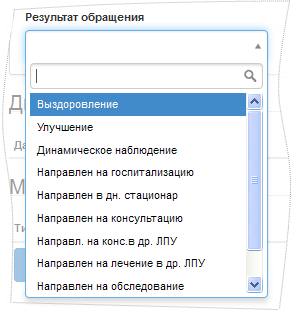
\includegraphics[width = 0.4\textwidth ,keepaspectratio]{gen_filtr}
 	\caption{Поле поиска \slash фильтрации данных справочника}
 	\label{img_gen_filtr}
 \end{figure} 
 
 \item При раскрытии справочника курсор автоматически помещается в поле поиска. Можно сразу начинать ввод строки поиска.
 \item Фильтрация производится по мере ввода текста в поле поиска. Т.е. состав элементов справочника меняется при вводе каждого нового символа в поле поиска. Нажатия дополнительных кнопок для запуска поиска не требуется.
 \item В результаты поиска попадают записи, содержащие введенный текст. Текст может находиться в любом месте записи (не обязательно в начале наименования или слова).
 \item Регистр букв не учитывается при поиске.
 \item В активной записи найденная строка выделется цветом (Рисунок \ref{img_gen_filtr2}).
 \item Для отмены фильтрации и получения полного справочника следует очистить поле поиска.
\end{itemize} 

\begin{figure}[!ht]\centering
	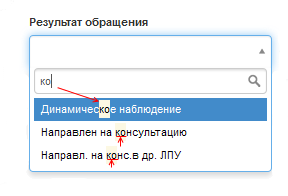
\includegraphics[width = 0.4\textwidth ,keepaspectratio]{gen_filtr2}
	\caption{Применение фильтрации данных}
	\label{img_gen_filtr2}
\end{figure}  

\subsubsection{Работа с элементом управления <<Календарь>>} \label{gen_cal}

Элемент управления <<Календарь>> используется во всех полях, содержащих дату, в системе. На некоторых страницах (например, при работе с расписанием) он находится постоянно в раскрытом виде, в других случаях раскрывается по нажатию кнопки 
\includegraphics[scale=0.6]{cal} справа от соответствующего поля либо установке курсора в поле для ввода даты. Во всех случаях принцип работы с календарем одинаков.

Для выбора даты из календаря, достаточно щелкнуть по нужному числу месяца в календаре левой кнопкой мыши.  Как правило, по умолчанию в календаре открывается текущий месяц и выбирается текущий день. Если в поле размещения календаря уже введена какая-то дата, то календарь открывается на месяце указанного года, к которому относится дата. Если календарь привязан к полю ввода даты, то можно ввести дату с клавиатуры (достаточно ввести только цифры, без разделителей). Разделители будут подставлены автоматически в соответствии с форматом даты. При этом в календаре будет автоматически выбрана введенная дата.

Для перехода по месяцам можно использовать стрелки, расположенные справа и слева от названия месяца в верхней части календаря (Рисунок \ref{img_gen_caldrill}). При нажатии на стрелки будет осуществляться переход к следующему или предыдущему месяцу соответственно.

\begin{figure}[!ht]\centering
	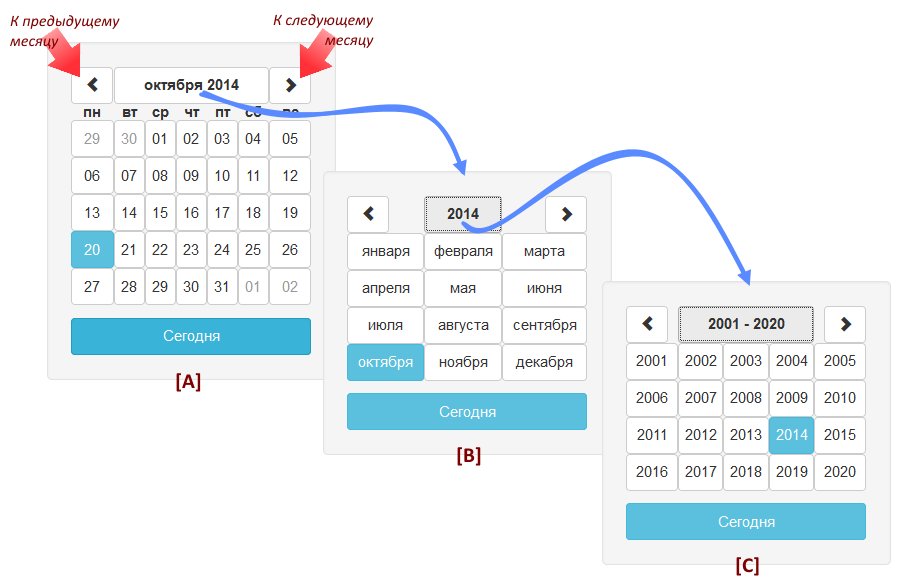
\includegraphics[width = 0.8\textwidth ,keepaspectratio]{gen_caldrill}
	\caption{Механизм работы календаря}
	\label{img_gen_caldrill}
\end{figure} 

Можно выбрать произвольный месяц из календаря. Для этого следует нажать на кнопку с названием месяца в верхней части календаря. После этого календарь примет вид [B] (Рисунок \ref{img_gen_caldrill}). В верхней части календаря будет указан номер года. Стрелки, расположенные слева и справа от номера года, позволяют перейти к предыдущему или следующему году. Щелчок левой кнопкой мыши по названию месяца позволяет раскрыть числа этого месяца.

При нажатии на кнопку с номером года в верхней части календаря, он примет вид [C] (Рисунок \ref{img_gen_caldrill}). В основной части календаря будут отображаться номера лет текущего двадцатилетия. Переход к следующему или предыдущему двадцатилетию осуществляется при нажатии на кнопки, расположенные слева и справа от кнопки, содержащей интервалы лет. При нажатии на кнопку с интервалами лет осуществляется возврат к текущему месяцу (вид [A]). Для выбора даты в календаре вида С следует щелкнуть левой кнопкой мыши по номеру нужного года, далее в видоизменившемся календаре вида В выбрать месяц, и затем - число месяца.
 
Для быстрого возврата к просмотру текущего дня либо установки текущей даты в поле ввода предусмотрена кнопка \btn{Сегодня} в нижней части календаря. 

При раскрытии календаря в поле ввода в нем появляются так же дополнительные кнопки:

\begin{itemize}
	\item \btn{Недели} -- позволяет скрывать и отображать номера недель в крайнем левом столбце календаря. Кнопка работает по принципу переключателя: если первое нажатие скрывает номера недель, то повторное - снова их отображает.
	\item \btn{Убрать} -- скрывает календарь и очищает поле ввода даты.
	\item \btn{Готово} -- скрывает календарь, сохраняя при этом введенное в поле значение. 
\end{itemize}